% Author: Izaak Neutelings (July 2021)
% Description: ttbar & ttH jets
% Inspiration: PhD thesis by Korbinian Schweiger
\documentclass[border=3pt,tikz]{standalone}
\usepackage{amsmath}
\usepackage{physics}
\usepackage{xcolor}
\usetikzlibrary{calc}
\usetikzlibrary{math} % for \tikzmath
\tikzset{>=latex} % for LaTeX arrow head
\usetikzlibrary{decorations.pathreplacing} % for curly braces

\colorlet{myred}{red!70!black}
\colorlet{mydarkred}{red!45!black}
\colorlet{myblue}{blue!70!black}
\colorlet{mydarkblue}{blue!40!black}
\colorlet{mygreen}{green!80!black}
\colorlet{mydarkgreen}{green!50!black}
\colorlet{mypurple}{blue!50!red!80!black}
\colorlet{myorange}{orange!70!red!80!black}
\colorlet{mydarkorange}{orange!70!red!70!black}
\tikzstyle{vector}=[->,very thick,myblue,line cap=round]
\tikzstyle{ptmiss}=[->,dashed,thick,myred,line cap=round]
\tikzstyle{cone}=[thin,blue!50!black,fill=blue!50!black!30] %,fill opacity=0.8
\tikzstyle{conebase}=[cone,fill=blue!50!black!50] %,fill opacity=0.8
\tikzstyle{loose dashed}=[dash pattern=on 5pt off 5pt]

\newcommand{\qbar}{{\ensuremath{\overline{q}}}} %\xspace
\newcommand{\bbar}{{\ensuremath{\overline{\mathrm{b}}}}} %\xspace
\newcommand\jetcone[5][blue]{{
  \pgfmathanglebetweenpoints{\pgfpointanchor{#2}{center}}{\pgfpointanchor{#3}{center}}
  \edef\ang{#4/2} % half-opening angle
  \edef\e{#5} % ratio a/b ("eccentricity") of cone top
  \edef\vang{\pgfmathresult} % angle of vector OV
  \coordinate (tmpO) at ($(#2)+(\vang:0.017)$); % shift origin due to sharp point
  \tikzmath{
    coordinate \C;
    \C = (tmpO)-(#3); % vector OV
    \x = veclen(\Cx,\Cy)*\e*sin(\ang)^2; % x coordinate P
    \y = tan(\ang)*(veclen(\Cx,\Cy)-\x); % y coordinate P
    \a = veclen(\Cx,\Cy)*sqrt(\e)*sin(\ang); % vertical radius
    \b = veclen(\Cx,\Cy)*tan(\ang)*sqrt(1-\e*sin(\ang)^2); % horizontal radius
    \angb = acos(sqrt(\e)*sin(\ang)); % angle of P in ellipse
  }
  \coordinate (tmpL) at ($(#3)-(\vang:\x pt)+(\vang+90:\y pt)$); % tangency
  \draw[thin,#1!40!black,rotate=\vang, %,fill=#1!50!black!80
    top color=#1!50!black!80,bottom color=#1!40!black!80,shading angle=\vang]
    (#3) ellipse({\a pt} and {\b pt});
  \draw[thin,#1!40!black,rotate=\vang,%fill=#1!80!black!40,
  top color=#1!90!black!20,bottom color=#1!50!black!50,shading angle=\vang]
    (tmpL) arc(180-\angb:180+\angb:{\a pt} and {\b pt})
    -- (tmpO) -- cycle;
}}


\begin{document}


% TTBAR JETS - no text
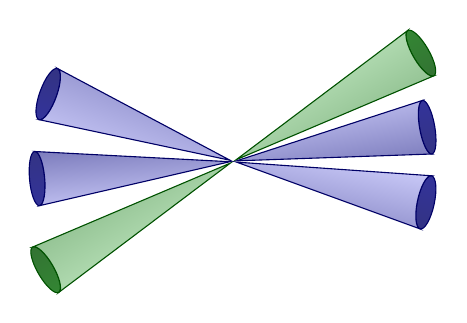
\begin{tikzpicture}[scale=2.5]
  \def\R{1} % scale jet length
  \coordinate (O) at (0,0);
  \coordinate (B1) at (  30:1.1*\R); % b jet 1 (top)
  \coordinate (J1) at (  10:1.0*\R); % q jet 1 (top)
  \coordinate (J2) at ( -12:1.0*\R); % q jet 2 (top)
  \coordinate (B2) at (-150:1.1*\R); % b jet 2 (antitop)
  \coordinate (J3) at ( 185:1.0*\R); % q jet 3 (antitop)
  \coordinate (J4) at ( 160:1.0*\R); % q jet 4 (antitop)
  
  % TOP 1
  \jetcone[mygreen]{O}{B1}{14}{0.10}
  \jetcone{O}{J1}{16}{0.08}
  \jetcone{O}{J2}{16}{0.10}
  
  % TOP 2
  \jetcone[mygreen]{O}{B2}{14}{0.10}
  \jetcone{O}{J3}{16}{0.08}
  \jetcone{O}{J4}{16}{0.10}
  
\end{tikzpicture}


% TTBAR JETS 
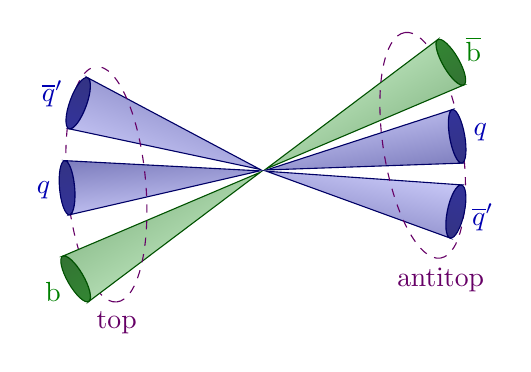
\begin{tikzpicture}[scale=2.5]
  \def\R{1} % scale jet length
  \coordinate (O) at (0,0);
  \coordinate (B1) at (  30:1.1*\R); % b jet 1 (top)
  \coordinate (J1) at (  10:1.0*\R); % q jet 1 (top)
  \coordinate (J2) at ( -12:1.0*\R); % q jet 2 (top)
  \coordinate (B2) at (-150:1.1*\R); % b jet 2 (antitop)
  \coordinate (J3) at ( 185:1.0*\R); % q jet 3 (antitop)
  \coordinate (J4) at ( 160:1.0*\R); % q jet 4 (antitop)
  
  % TOP 1
  \def\tang{9}
  \draw[dashed,mypurple,rotate=\tang]
    ($(O)+(0.82*\R,0.58*\R)$) arc(90:-90:{0.2*\R} and {0.58*\R});
  \jetcone[mygreen]{O}{B1}{14}{0.10}
  \jetcone{O}{J1}{16}{0.08}
  \jetcone{O}{J2}{16}{0.10}
  \draw[dashed,mypurple,rotate=\tang]
    ($(O)+(0.82*\R,0.58*\R)$) arc(90:270:{0.2*\R} and {0.58*\R})
    node[below] {antitop};
  \node[mydarkgreen] at ($(O)!1.12!(B1)$) {\bbar};
  \node[myblue] at ($(O)!1.12!(J1)$) {$q$};
  \node[myblue] at ($(O)!1.14!(J2)$) {$\qbar'$};
  
  % TOP 2
  \def\tang{185}
  \draw[dashed,mypurple,rotate=\tang]
    ($(O)+(0.8*\R,0.6*\R)$) arc(90:-90:{0.2*\R} and {0.6*\R});
  \jetcone[mygreen]{O}{B2}{14}{0.10}
  \jetcone{O}{J3}{16}{0.08}
  \jetcone{O}{J4}{16}{0.10}
  \draw[dashed,mypurple,rotate=\tang]
    ($(O)+(0.8*\R,0.6*\R)$) arc(90:270:{0.2*\R} and {0.6*\R})
    node[pos=0,below] {top};
  \node[mydarkgreen] at ($(O)!1.12!(B2)$) {b};
  \node[myblue] at ($(O)!1.12!(J3)$) {$q$};
  \node[myblue] at ($(O)!1.14!(J4)$) {$\qbar'$};
  
\end{tikzpicture}


% TTBAR JETS 
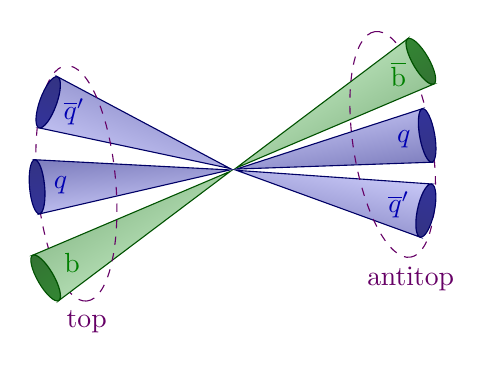
\begin{tikzpicture}[scale=2.5]
  \def\R{1} % scale jet length
  \coordinate (O) at (0,0);
  \coordinate (B1) at (  30:1.1*\R); % b jet 1 (top)
  \coordinate (J1) at (  10:1.0*\R); % q jet 1 (top)
  \coordinate (J2) at ( -12:1.0*\R); % q jet 2 (top)
  \coordinate (B2) at (-150:1.1*\R); % b jet 2 (antitop)
  \coordinate (J3) at ( 185:1.0*\R); % q jet 3 (antitop)
  \coordinate (J4) at ( 160:1.0*\R); % q jet 4 (antitop)
  
  % TOP 1
  \def\tang{9}
  \draw[dashed,mypurple,rotate=\tang]
    ($(O)+(0.82*\R,0.58*\R)$) arc(90:-90:{0.2*\R} and {0.58*\R});
  \jetcone[mygreen]{O}{B1}{14}{0.10}
  \jetcone{O}{J1}{16}{0.08}
  \jetcone{O}{J2}{16}{0.10}
  \draw[dashed,mypurple,rotate=\tang]
    ($(O)+(0.82*\R,0.58*\R)$) arc(90:270:{0.2*\R} and {0.58*\R})
    node[below] {antitop};
  \node[mydarkgreen] at ($(O)!0.88!(B1)$) {\bbar};
  \node[myblue] at ($(O)!0.88!(J1)$) {$q$};
  \node[myblue] at ($(O)!0.86!(J2)$) {$\qbar'$};
  
  % TOP 2
  \def\tang{185}
  \draw[dashed,mypurple,rotate=\tang]
    ($(O)+(0.8*\R,0.6*\R)$) arc(90:-90:{0.2*\R} and {0.6*\R});
  \jetcone[mygreen]{O}{B2}{14}{0.10}
  \jetcone{O}{J3}{16}{0.08}
  \jetcone{O}{J4}{16}{0.10}
  \draw[dashed,mypurple,rotate=\tang]
    ($(O)+(0.8*\R,0.6*\R)$) arc(90:270:{0.2*\R} and {0.6*\R})
    node[pos=0,below] {top};
  \node[mydarkgreen] at ($(O)!0.86!(B2)$) {b};
  \node[myblue] at ($(O)!0.88!(J3)$) {$q$};
  \node[myblue] at ($(O)!0.86!(J4)$) {$\qbar'$};
  
\end{tikzpicture}


% TTBAR JETS - semileptonic
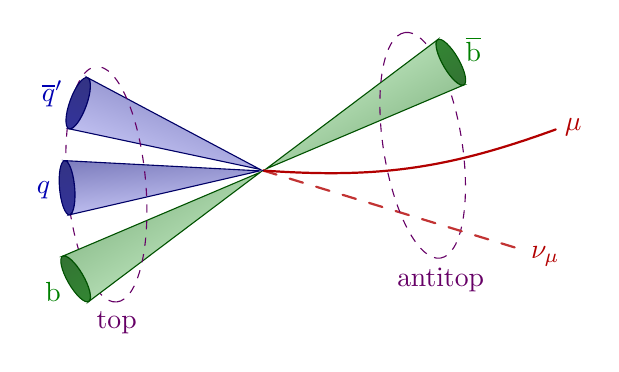
\begin{tikzpicture}[scale=2.5]
  \def\R{1} % scale jet length
  \coordinate (O) at (0,0);
  \coordinate (B1) at (  30:1.1*\R); % b jet 1 (top)
  \coordinate (M1) at (   8:1.5*\R); % muon (top)
  \coordinate (N1) at ( -17:1.4*\R); % neutrino (top)
  \coordinate (B2) at (-150:1.1*\R); % b jet 2 (antitop)
  \coordinate (J3) at ( 185:1.0*\R); % q jet 3 (antitop)
  \coordinate (J4) at ( 160:1.0*\R); % q jet 4 (antitop)
  
  % TOP 1
  \def\tang{9}
  \draw[dashed,mypurple,rotate=\tang]
    ($(O)+(0.82*\R,0.58*\R)$) arc(90:-90:{0.2*\R} and {0.58*\R});
  \jetcone[mygreen]{O}{B1}{14}{0.10}
  %\jetcone[myred!50!white]{O}{M1}{6}{0.08}
  \draw[loose dashed,thick,myred!80,line cap=round] (O) -- (N1);
  \draw[myred,thick,line cap=round] (O) to[out=-4,in=-160] (M1);
  \draw[dashed,mypurple,rotate=\tang]
    ($(O)+(0.82*\R,0.58*\R)$) arc(90:270:{0.2*\R} and {0.58*\R})
    node[below] {antitop};
  \node[mydarkgreen] at ($(O)!1.12!(B1)$) {\bbar};
  \node[myred] at ($(O)!1.06!(M1)$) {$\mu$};
  \node[myred] at ($(O)!1.07!(N1)$) {$\nu_\mu$};
  
  % TOP 2
  \def\tang{185}
  \draw[dashed,mypurple,rotate=\tang]
    ($(O)+(0.8*\R,0.6*\R)$) arc(90:-90:{0.2*\R} and {0.6*\R});
  \jetcone[mygreen]{O}{B2}{14}{0.10}
  \jetcone{O}{J3}{16}{0.08}
  \jetcone{O}{J4}{16}{0.10}
  \draw[dashed,mypurple,rotate=\tang]
    ($(O)+(0.8*\R,0.6*\R)$) arc(90:270:{0.2*\R} and {0.6*\R})
    node[pos=0,below] {top};
  \node[mydarkgreen] at ($(O)!1.12!(B2)$) {b};
  \node[myblue] at ($(O)!1.12!(J3)$) {$q$};
  \node[myblue] at ($(O)!1.14!(J4)$) {$\qbar'$};
  
\end{tikzpicture}


% TTBAR JETS - recoiling 1
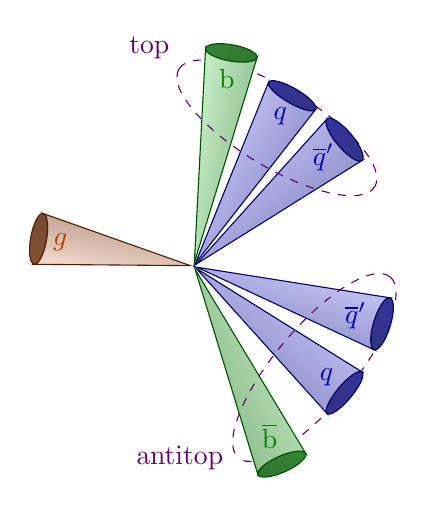
\begin{tikzpicture}[scale=2.5]
  \def\R{1} % scale jet length
  \coordinate (O) at (0,0);
  \coordinate (B1) at ( 80:1.1*\R); % b jet 1 (top)
  \coordinate (J1) at ( 60:1.0*\R); % q jet 1 (top)
  \coordinate (J2) at ( 40:1.0*\R); % q jet 2 (top)
  \coordinate (B2) at (-66:1.1*\R); % b jet 2 (antitop)
  \coordinate (J3) at (-40:1.0*\R); % q jet 3 (antitop)
  \coordinate (J4) at (-17:1.0*\R); % q jet 4 (antitop)
  \coordinate (G1) at (170:0.8*\R); % gluon (ISR/FSR)
  
  % TOP 1
  \def\tang{59}
  \draw[dashed,mypurple,rotate=\tang]
    ($(O)+(0.82*\R,0.58*\R)$) arc(90:-90:{0.2*\R} and {0.58*\R});
  \jetcone[mygreen]{O}{B1}{14}{0.10}
  \jetcone{O}{J1}{16}{0.08}
  \jetcone{O}{J2}{16}{0.10}
  \draw[dashed,mypurple,rotate=\tang]
    ($(O)+(0.82*\R,0.58*\R)$) arc(90:270:{0.2*\R} and {0.58*\R})
    node[pos=0,above left=0] {top};
  \node[mydarkgreen] at ($(O)!0.88!(B1)$) {b};
  \node[myblue] at ($(O)!0.88!(J1)$) {$q$};
  \node[myblue] at ($(O)!0.86!(J2)$) {$\qbar'$};
  
  % TOP 2
  \def\tang{-40}
  \draw[dashed,mypurple,rotate=\tang]
    ($(O)+(0.8*\R,0.6*\R)$) arc(90:-90:{0.2*\R} and {0.6*\R});
  \jetcone[mygreen]{O}{B2}{14}{0.10}
  \jetcone{O}{J3}{16}{0.08}
  \jetcone{O}{J4}{16}{0.10}
  \draw[dashed,mypurple,rotate=\tang]
    ($(O)+(0.8*\R,0.6*\R)$) arc(90:270:{0.2*\R} and {0.6*\R})
    node[left=2] {antitop};
  \node[mydarkgreen] at ($(O)!0.86!(B2)$) {\bbar};
  \node[myblue] at ($(O)!0.88!(J3)$) {$q$};
  \node[myblue] at ($(O)!0.86!(J4)$) {$\qbar'$};
  
  % GLUON
  \jetcone[myorange]{O}{G1}{19}{0.10}
  \node[mydarkorange] at ($(O)!0.86!(G1)$) {$g$};
  
\end{tikzpicture}


% TTBAR JETS - recoiling 2
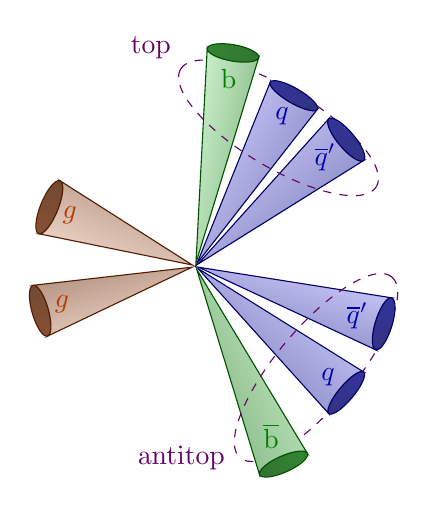
\begin{tikzpicture}[scale=2.5]
  \def\R{1} % scale jet length
  \coordinate (O) at (0,0);
  \coordinate (B1) at ( 80:1.1*\R); % b jet 1 (top)
  \coordinate (J1) at ( 60:1.0*\R); % q jet 1 (top)
  \coordinate (J2) at ( 40:1.0*\R); % q jet 2 (top)
  \coordinate (B2) at (-66:1.1*\R); % b jet 2 (antitop)
  \coordinate (J3) at (-40:1.0*\R); % q jet 3 (antitop)
  \coordinate (J4) at (-17:1.0*\R); % q jet 4 (antitop)
  \coordinate (G1) at (158:0.80*\R); % gluon 1 (ISR/FSR)
  \coordinate (G2) at (196:0.82*\R); % gluon 2 (ISR/FSR)
  
  % TOP 1
  \def\tang{59}
  \draw[dashed,mypurple,rotate=\tang]
    ($(O)+(0.82*\R,0.58*\R)$) arc(90:-90:{0.2*\R} and {0.58*\R});
  \jetcone[mygreen]{O}{B1}{14}{0.10}
  \jetcone{O}{J1}{16}{0.08}
  \jetcone{O}{J2}{16}{0.10}
  \draw[dashed,mypurple,rotate=\tang]
    ($(O)+(0.82*\R,0.58*\R)$) arc(90:270:{0.2*\R} and {0.58*\R})
    node[pos=0,above left=0] {top};
  \node[mydarkgreen] at ($(O)!0.88!(B1)$) {b};
  \node[myblue] at ($(O)!0.88!(J1)$) {$q$};
  \node[myblue] at ($(O)!0.86!(J2)$) {$\qbar'$};
  
  % TOP 2
  \def\tang{-40}
  \draw[dashed,mypurple,rotate=\tang]
    ($(O)+(0.8*\R,0.6*\R)$) arc(90:-90:{0.2*\R} and {0.6*\R});
  \jetcone[mygreen]{O}{B2}{14}{0.10}
  \jetcone{O}{J3}{16}{0.08}
  \jetcone{O}{J4}{16}{0.10}
  \draw[dashed,mypurple,rotate=\tang]
    ($(O)+(0.8*\R,0.6*\R)$) arc(90:270:{0.2*\R} and {0.6*\R})
    node[left=2] {antitop};
  \node[mydarkgreen] at ($(O)!0.86!(B2)$) {\bbar};
  \node[myblue] at ($(O)!0.88!(J3)$) {$q$};
  \node[myblue] at ($(O)!0.86!(J4)$) {$\qbar'$};
  
  % GLUON
  \jetcone[myorange]{O}{G1}{21}{0.10}
  \jetcone[myorange]{O}{G2}{19}{0.10}
  \node[mydarkorange] at ($(O)!0.86!(G1)$) {$g$};
  \node[mydarkorange] at ($(O)!0.86!(G2)$) {$g$};
  
\end{tikzpicture}


% TTBAR JETS - recoiling 3 (no text)
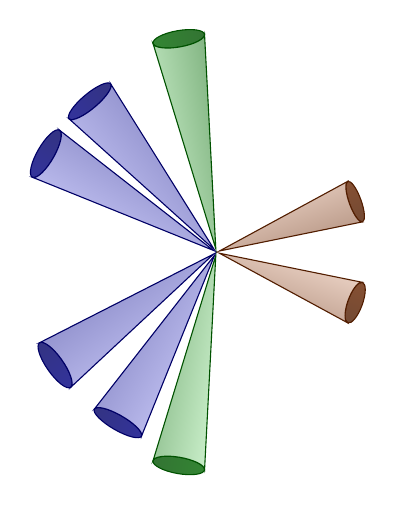
\begin{tikzpicture}[scale=2.5]
  \def\R{1} % scale jet length
  \coordinate (O) at (0,0);
  \coordinate (B1) at ( 100:1.1*\R); % b jet 1
  \coordinate (J1) at ( 130:1.0*\R); % q jet 1
  \coordinate (J2) at ( 150:1.0*\R); % q jet 2
  \coordinate (B2) at (-100:1.1*\R); % b jet 2
  \coordinate (J3) at (-120:1.0*\R); % q jet 3
  \coordinate (J4) at (-145:1.0*\R); % q jet 4
  \coordinate (R1) at (  20:0.75*\R); % recoil jet 1
  \coordinate (R2) at ( -20:0.75*\R); % recoil jet 2
  
  % TOP 1
  \jetcone[mygreen]{O}{B1}{14}{0.10}
  \jetcone{O}{J1}{16}{0.08}
  \jetcone{O}{J2}{16}{0.10}
  
  % TOP 2
  \jetcone[mygreen]{O}{B2}{14}{0.10}
  \jetcone{O}{J3}{16}{0.08}
  \jetcone{O}{J4}{16}{0.10}
  
  % RECOIL
  \jetcone[myorange]{O}{R1}{17}{0.08}
  \jetcone[myorange]{O}{R2}{17}{0.12}
  
\end{tikzpicture}


% ttH JETS - no text
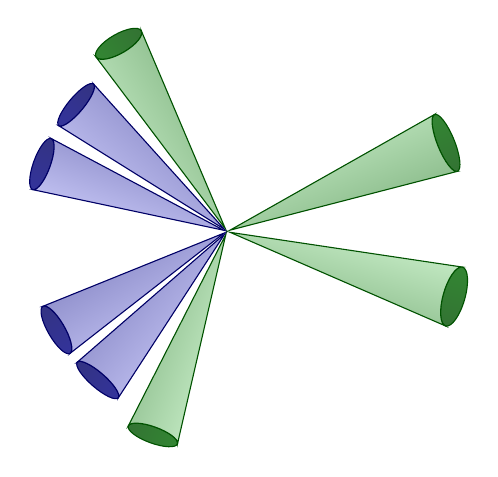
\begin{tikzpicture}[scale=2.5]
  \def\R{1} % scale jet length
  \coordinate (O) at (0,0);
  \coordinate (B1) at ( 120:1.1*\R); % b jet 1 (top)
  \coordinate (J1) at ( 140:1.0*\R); % q jet 1 (top)
  \coordinate (J2) at ( 160:1.0*\R); % q jet 2 (top)
  \coordinate (B2) at (-110:1.1*\R); % b jet 2 (antitop)
  \coordinate (J3) at (-131:1.0*\R); % q jet 3 (antitop)
  \coordinate (J4) at (-150:1.0*\R); % q jet 4 (antitop)
  \coordinate (H1) at (  22:1.2*\R); % b jet 3 (Higgs)
  \coordinate (H2) at ( -16:1.2*\R); % b jet 4 (Higgs)
  
  % TOP 1
  \jetcone[mygreen]{O}{B1}{14}{0.14}
  \jetcone{O}{J1}{16}{0.08}
  \jetcone{O}{J2}{16}{0.10}
  
  % TOP 2
  \jetcone[mygreen]{O}{B2}{14}{0.10}
  \jetcone{O}{J3}{16}{0.08}
  \jetcone{O}{J4}{16}{0.10}
  
  % HIGGS
  \jetcone[mygreen]{O}{H1}{15}{0.08}
  \jetcone[mygreen]{O}{H2}{15}{0.13}
  
\end{tikzpicture}


% ttH JETS
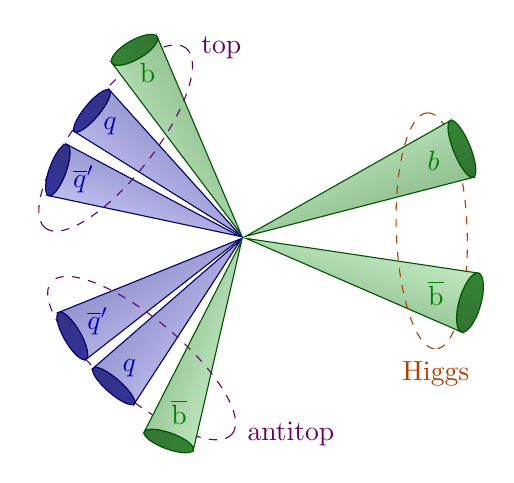
\begin{tikzpicture}[scale=2.5]
  \def\R{1} % scale jet length
  \coordinate (O) at (0,0);
  \coordinate (B1) at ( 120:1.1*\R); % b jet 1 (top)
  \coordinate (J1) at ( 140:1.0*\R); % q jet 1 (top)
  \coordinate (J2) at ( 160:1.0*\R); % q jet 2 (top)
  \coordinate (B2) at (-110:1.1*\R); % b jet 2 (antitop)
  \coordinate (J3) at (-131:1.0*\R); % q jet 3 (antitop)
  \coordinate (J4) at (-150:1.0*\R); % q jet 4 (antitop)
  \coordinate (H1) at (  22:1.2*\R); % b jet 3 (Higgs)
  \coordinate (H2) at ( -16:1.2*\R); % b jet 4 (Higgs)
  
  % TOP 1
  \def\tang{142}
  \draw[dashed,mypurple,rotate=\tang]
    ($(O)+(0.82*\R,0.58*\R)$) arc(90:-90:{0.2*\R} and {0.58*\R});
  \jetcone[mygreen]{O}{B1}{14}{0.14}
  \jetcone{O}{J1}{16}{0.08}
  \jetcone{O}{J2}{16}{0.10}
  \draw[dashed,mypurple,rotate=\tang]
    ($(O)+(0.82*\R,0.58*\R)$) arc(90:270:{0.2*\R} and {0.58*\R})
    node[right=2] {top};
  \node[mydarkgreen] at ($(O)!0.88!(B1)$) {b};
  \node[myblue] at ($(O)!0.88!(J1)$) {$q$};
  \node[myblue] at ($(O)!0.86!(J2)$) {$\qbar'$};
  
  % TOP 2
  \def\tang{-130}
  \draw[dashed,mypurple,rotate=\tang]
    ($(O)+(0.8*\R,0.6*\R)$) arc(90:-90:{0.2*\R} and {0.6*\R});
  \jetcone[mygreen]{O}{B2}{14}{0.10}
  \jetcone{O}{J3}{16}{0.08}
  \jetcone{O}{J4}{16}{0.10}
  \draw[dashed,mypurple,rotate=\tang]
    ($(O)+(0.8*\R,0.6*\R)$) arc(90:270:{0.2*\R} and {0.6*\R})
    node[pos=0,right=2] {antitop};
  \node[mydarkgreen] at ($(O)!0.86!(B2)$) {\bbar};
  \node[myblue] at ($(O)!0.88!(J3)$) {$q$};
  \node[myblue] at ($(O)!0.85!(J4)$) {$\qbar'$};
  
  % HIGGS
  \def\tang{2}
  \draw[dashed,mydarkorange,rotate=\tang]
    ($(O)+(0.96*\R,0.6*\R)$) arc(90:-90:{0.18*\R} and {0.6*\R});
  \jetcone[mygreen]{O}{H1}{15}{0.08}
  \jetcone[mygreen]{O}{H2}{15}{0.13}
  \draw[dashed,mydarkorange,rotate=\tang]
    ($(O)+(0.96*\R,0.6*\R)$) arc(90:270:{0.18*\R} and {0.6*\R})
    node[below=1] {Higgs};
  \node[mydarkgreen] at ($(O)!0.87!(H1)$) {$b$};
  \node[mydarkgreen] at ($(O)!0.85!(H2)$) {$\bbar$};
  
\end{tikzpicture}


% ttH JETS - recoil
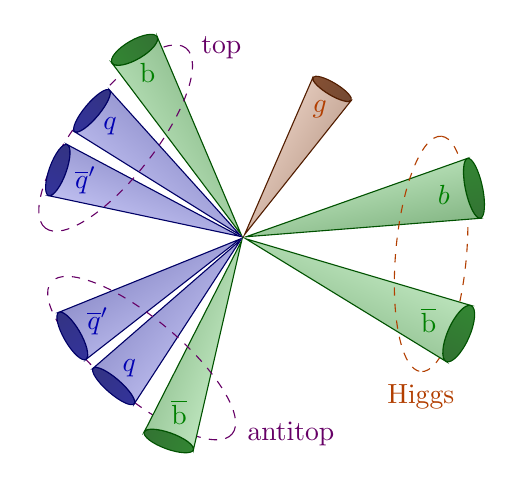
\begin{tikzpicture}[scale=2.5]
  \def\R{1} % scale jet length
  \coordinate (O) at (0,0);
  \coordinate (B1) at ( 120:1.1*\R); % b jet 1 (top)
  \coordinate (J1) at ( 140:1.0*\R); % q jet 1 (top)
  \coordinate (J2) at ( 160:1.0*\R); % q jet 2 (top)
  \coordinate (B2) at (-110:1.1*\R); % b jet 2 (antitop)
  \coordinate (J3) at (-131:1.0*\R); % q jet 3 (antitop)
  \coordinate (J4) at (-150:1.0*\R); % q jet 4 (antitop)
  \coordinate (H1) at (  12:1.2*\R); % b jet 3 (Higgs)
  \coordinate (H2) at ( -24:1.2*\R); % b jet 4 (Higgs)
  \coordinate (G1) at (  59:0.88*\R); % gluon
  
  % TOP 1
  \def\tang{142}
  \draw[dashed,mypurple,rotate=\tang]
    ($(O)+(0.82*\R,0.58*\R)$) arc(90:-90:{0.2*\R} and {0.58*\R});
  \jetcone[mygreen]{O}{B1}{14}{0.14}
  \jetcone{O}{J1}{16}{0.08}
  \jetcone{O}{J2}{16}{0.10}
  \draw[dashed,mypurple,rotate=\tang]
    ($(O)+(0.82*\R,0.58*\R)$) arc(90:270:{0.2*\R} and {0.58*\R})
    node[right=2] {top};
  \node[mydarkgreen] at ($(O)!0.88!(B1)$) {b};
  \node[myblue] at ($(O)!0.88!(J1)$) {$q$};
  \node[myblue] at ($(O)!0.85!(J2)$) {$\qbar'$};
  
  % TOP 2
  \def\tang{-130}
  \draw[dashed,mypurple,rotate=\tang]
    ($(O)+(0.8*\R,0.6*\R)$) arc(90:-90:{0.2*\R} and {0.6*\R});
  \jetcone[mygreen]{O}{B2}{14}{0.10}
  \jetcone{O}{J3}{16}{0.08}
  \jetcone{O}{J4}{16}{0.10}
  \draw[dashed,mypurple,rotate=\tang]
    ($(O)+(0.8*\R,0.6*\R)$) arc(90:270:{0.2*\R} and {0.6*\R})
    node[pos=0,right=2] {antitop};
  \node[mydarkgreen] at ($(O)!0.86!(B2)$) {\bbar};
  \node[myblue] at ($(O)!0.88!(J3)$) {$q$};
  \node[myblue] at ($(O)!0.85!(J4)$) {$\qbar'$};
  
  % HIGGS
  \def\tang{-5}
  \draw[dashed,mydarkorange,rotate=\tang]
    ($(O)+(0.96*\R,0.6*\R)$) arc(90:-90:{0.18*\R} and {0.6*\R});
  \jetcone[mygreen]{O}{H1}{15}{0.08}
  \jetcone[mygreen]{O}{H2}{15}{0.13}
  \draw[dashed,mydarkorange,rotate=\tang]
    ($(O)+(0.96*\R,0.6*\R)$) arc(90:270:{0.18*\R} and {0.6*\R})
    node[below=1] {Higgs};
  \node[mydarkgreen] at ($(O)!0.87!(H1)$) {$b$};
  \node[mydarkgreen] at ($(O)!0.86!(H2)$) {$\bbar$};
  
  % RECOIL
  \jetcone[myorange]{O}{G1}{15}{0.08}
  \node[mydarkorange] at ($(O)!0.86!(G1)$) {$g$};
  
\end{tikzpicture}


\end{document}